\documentclass[a4paper,12pt]{article}
\usepackage[T1]{fontenc}
\usepackage{imakeidx}
\usepackage{graphicx}
%\makeindex[columns=3, title=Alphabetical Index, intoc]

\begin{document}

\textbf{Daniele Della Cioppa}

\textbf{Software Developer}

\tableofcontents
\clearpage

\section{Knowledge unit}

This is what I've been covering so far during the apprenticeship:

\begin{itemize}
\item {database development}
\item {application life cycle}
\item docker
\item github 
\item LateX
\item PostgreSQL
\item Linux
\item {iOS & Android development}
\end{itemize}
\clearpage

\subsection{iOS & Android development}
This is the stage I'm at so far with mobile development since this is being literally self taught

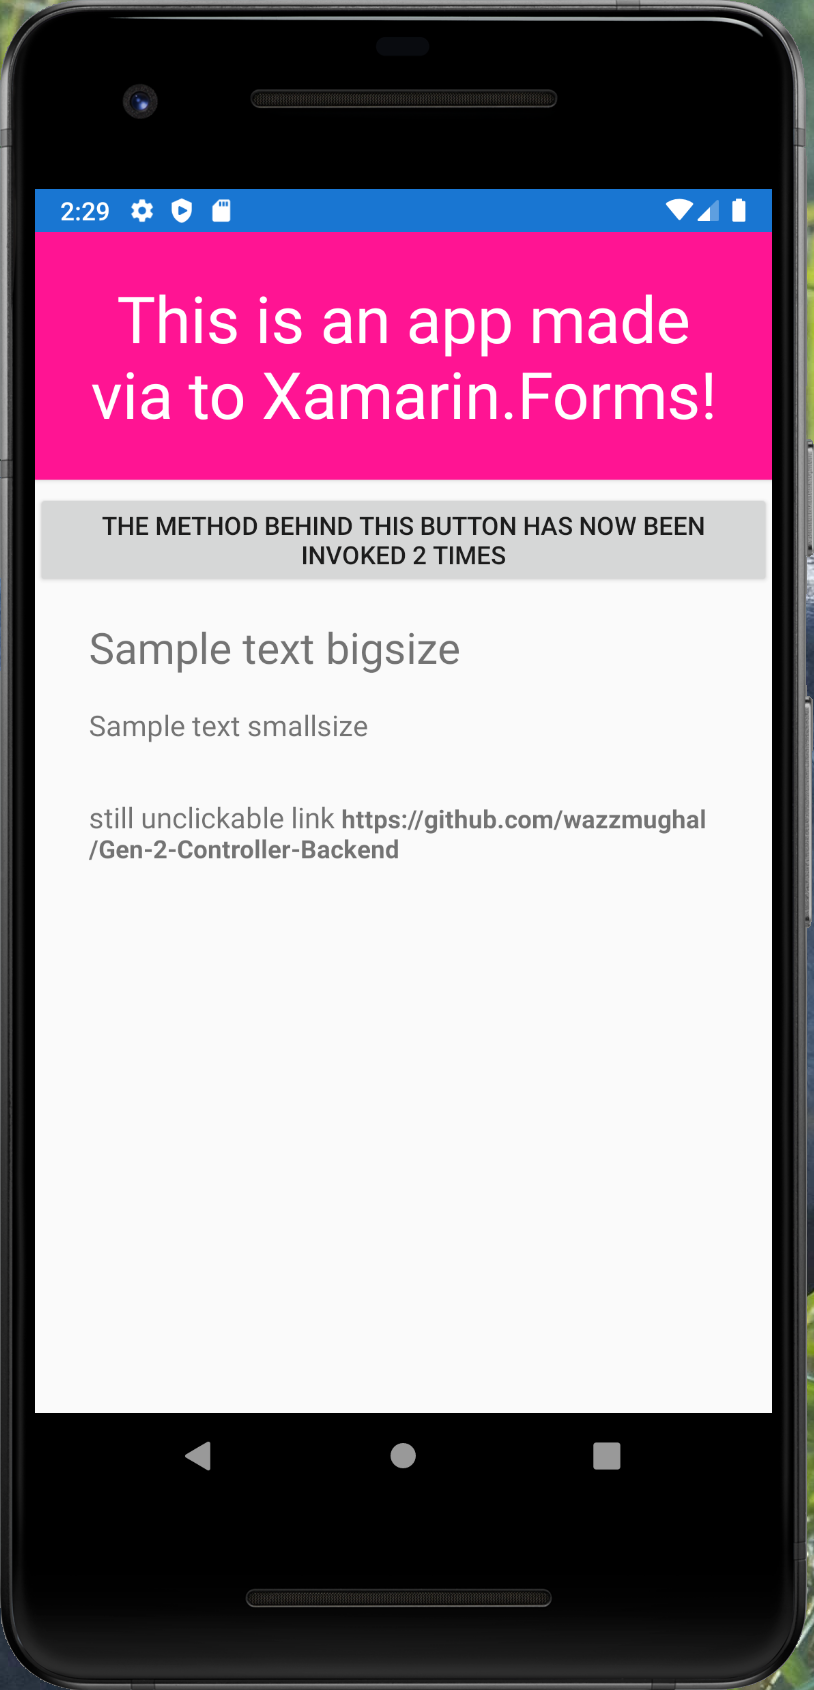
\includegraphics[width=9cm]{./capture-app.PNG}

 

\section{Introduction}

After three months in my role I'm now responsible for the following tasks with databases:

\begin{itemize}
\item {reading the specs}
\item design
\item implementation
\item testing 
\item documenting
\end{itemize}

\subsection{design}
\includegraphics[width=15cm]{./ERSchemaGen2.jpg}

\printindex

\end{document}
